\documentclass[fleqn, a4paper, 11pt, oneside]{amsart}
%\usepackage[top = 2cm, bottom = 1cm, left = 1cm, right = 1cm]{geometry}
\usepackage{exsheets, tasks}
\usepackage{amsmath, amssymb, amsthm} %standard AMS packages
\usepackage{marginnote} %marginnotes
\usepackage{gensymb} %miscellaneous symbols
\usepackage{commath} %differential symbols
\usepackage{xcolor} %colours
\usepackage{cancel} %cancelling terms
\usepackage{siunitx} %formatting units
\usepackage{tikz, pgfplots} %diagrams
\usetikzlibrary{calc, hobby, patterns, intersections}
\usepackage{graphicx} %inserting graphics
\usepackage{hyperref} %hyperlinks
\usepackage{datetime} %date and time
\usepackage{ulem} %underline for \emph{}
\usepackage{xfrac} %inline fractions
\usepackage{enumerate,enumitem} %numbered lists
\usepackage{float} %inserting floats
\usepackage{circuitikz} %circuit diagrams

\newcommand\numberthis{\addtocounter{equation}{1}\tag{\theequation}} %adds numbers to specific equations in non-numbered list of equations

\newcommand{\AxisRotator}[1][rotate=0]{
	\tikz [x=0.25cm,y=0.60cm,line width=.2ex,-stealth,#1] \draw (0,0) arc (-150:150:1 and 1);%
} %rotation symbols on axes

\theoremstyle{definition}
\newtheorem{example}{Example}
\newtheorem{definition}{Definition}

\theoremstyle{theorem}
\newtheorem{theorem}{Theorem}

\newcommand{\curl}{\mathrm{curl\,}}

\makeatletter
\@addtoreset{section}{part} %resets section numbers in new part
\makeatother

\renewcommand{\thesubsection}{(\arabic{subsection})}
\renewcommand{\thesection}{(\arabic{section})}

%section headings on left
\makeatletter
\def\specialsection{\@startsection{section}{1}%
	\z@{\linespacing\@plus\linespacing}{.5\linespacing}%
	%  {\normalfont\centering}}% DELETED
	{\normalfont}}% NEW
\def\section{\@startsection{section}{1}%
	\z@{.7\linespacing\@plus\linespacing}{.5\linespacing}%
	%  {\normalfont\scshape\centering}}% DELETED
	{\normalfont\scshape}}% NEW
\makeatother

%forces newline after subsection
\makeatletter
\def\subsection{\@startsection{subsection}{3}%
	\z@{.5\linespacing\@plus.7\linespacing}{.1\linespacing}%
	{\normalfont\itshape}}
\makeatother

\settasks{counter-format = tsk[1].}

\SetupExSheets{solution/print = true}

%opening
\title{Physics 2 : Assignment 4}
\author
{
	Aakash Jog\\
	ID : 989323563
}
\date{\formatdate{29}{4}{2015}}

\begin{document}

\maketitle
%\setlength{\mathindent}{0pt}

\begin{question}
	A metal sphere of radius $R$, carrying charge $q$, is surrounded by a thick concentric metal shell (inner radius $a$, outer radius $b$).
	The shell carries no net charge.
	\begin{enumerate}
		\item Find the surface charge density $a$ at $R$, at $a$, and at $b$.
		\item Find the potential at the center, using infinity as the reference point.
		\item
			Now the outer surface is touched to a grounding wire, which lowers its potential to zero (same as at infinity).
			How do your answers to the previous sub-questions change?
	\end{enumerate}
\end{question}

\begin{solution}
	\begin{enumerate}[leftmargin=*]
		\item 
			\begin{figure}[H]
				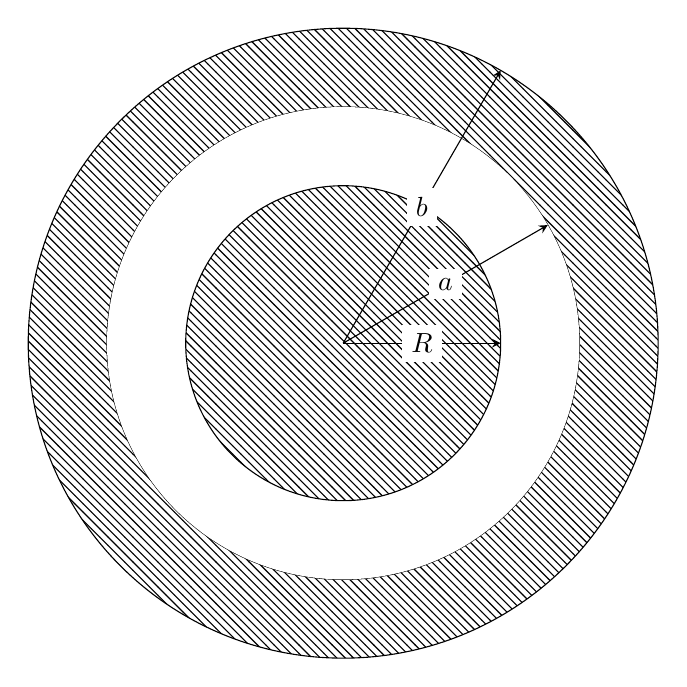
\begin{tikzpicture}
					\def\R{2};
					\def\a{3};
					\def\b{4};

					\begin{scope}
						\draw (0,0) circle (\b);
						\draw (0,0) circle (\a);

						\fill [pattern = north west lines] (0,0) circle (\b);
						\fill [color = white] (0,0) circle (\a);
					\end{scope}

					\begin{scope}
						\draw [fill, pattern = north west lines] (0,0) circle (\R);
					\end{scope}

					\begin{scope}[-stealth]
						\draw (0,0) -- ++(0:\R)  node [midway, fill = white] {$R$};
						\draw (0,0) -- ++(30:\a) node [midway, fill = white] {$a$};
						\draw (0,0) -- ++(60:\b) node [midway, fill = white] {$b$};
					\end{scope}
				\end{tikzpicture}
			\end{figure}
			Consider a spherical Gaussian surface with radius $r$, with $a < r < b$.
			By Gauss' Law, and as the electric field inside the thick metallic shell must be $0$, the net charge inside the Gaussian surface must be $0$.\\
			Therefore, the sum of the charge on the surface of the sphere and the charge on the inner surface of the shell must be $0$.
			Hence, the charge on the inner surface of the shell must be $-q$.\\
			As the shell is electrically neutral, the sum of the charges on the inner and outer surfaces of the shell must be $0$.
			Hence, the charge on the outer surface of the shell must be $q$.\\
			Therefore,
			\begin{align*}
				\sigma_R &= \dfrac{q}{4 \pi R^2}\\
				\sigma_a &= \dfrac{-q}{4 \pi a^2}\\
				\sigma_b &= \dfrac{q}{4 \pi b^2}
			\end{align*}
		\item
			\begin{align*}
				\varphi_{\textnormal{centre}} & = \textnormal{$\varphi$ due to charge at $R$} + \textnormal{$\varphi$ due to charge at $a$} + \textnormal{$\varphi$ due to charge at $b$} \\
                                                              & = \dfrac{q}{4 \pi \varepsilon_0 R}            + \dfrac{-q}{4 \pi \varepsilon_0 a}           + \dfrac{q}{4 \pi \varepsilon_0 b}
			\end{align*}
		\item
			\begin{align*}
				\varphi_b & = \textnormal{$\varphi$ due to charge at $R$} + \textnormal{$\varphi$ due to charge at $a$} + \textnormal{$\varphi$ due to charge at $b$} \\
                                          & = \dfrac{q}{4 \pi \varepsilon_0 b}            + \dfrac{-q}{4 \pi \varepsilon_0 b}           + \dfrac{q'}{4 \pi \varepsilon_0 b}                                \\
                                          & = \dfrac{q}{4 \pi \varepsilon_0 b}
			\end{align*}
			As the outer surface is grounded, its potential will be zero.\\
			Therefore
			\begin{align*}
				0             & = \dfrac{q'}{4 \pi \varepsilon_0 b} \\
				\therefore q' & = 0
			\end{align*}
			Therefore,
			\begin{align*}
				\sigma_R & = \dfrac{q}{4 \pi R^2}  \\
				\sigma_a & = \dfrac{-q}{4 \pi a^2} \\
				\sigma_b & = \dfrac{q'}{4 \pi b^2} \\
                                         & = 0
			\end{align*}
			\begin{align*}
				\varphi_{\textnormal{centre}} & = \textnormal{$\varphi$ due to charge at $R$} + \textnormal{$\varphi$ due to charge at $a$} + \textnormal{$\varphi$ due to charge at $b$} \\
                                                              & = \dfrac{q}{4 \pi \varepsilon_0 R}            + \dfrac{-q}{4 \pi \varepsilon_0 a}           + \dfrac{q'}{4 \pi \varepsilon_0 b}                                \\
                                                              & = \dfrac{q}{4 \pi \varepsilon_0 R}            + \dfrac{-q}{4 \pi \varepsilon_0 a}
			\end{align*}
	\end{enumerate}
\end{solution}

\begin{question}
	A metal sphere of radius $R$ carries a total charge $Q$.
	What is the force of repulsion between the ``northern'' hemisphere and the ``southern'' hemisphere?
\end{question}

\begin{solution}
	\begin{align*}
		E_{\textnormal{northern hemisphere}} &= \dfrac{1}{2} \dfrac{Q}{4 \pi \varepsilon_0 R^2}
	\end{align*}
	Due to the symmetry of the sphere, the components of the force of all elemental charges, in the direction of the north-south axis add up, and all other components cancel out.\\
	Therefore,
	\begin{align*}
		F & = \int\limits_{0}^{\frac{\pi}{2}} \int\limits_{0}^{2 \pi} E_{\textnormal{northern hemisphere}} \sigma R^2 \dif \varphi \sin(\theta) \cos(\theta) \dif \theta                                                       \\
                  & = \int\limits_{0}^{\frac{\pi}{2}} \int\limits_{0}^{2 \pi} \dfrac{1}{2} \cdot \dfrac{1}{4 \pi \varepsilon_0} \cdot \dfrac{Q}{R^2} \cdot \dfrac{Q}{4 \pi R^2} R^2 \sin(\theta) \cos(\theta) \dif \varphi \dif \theta \\
                  & = \int\limits_{0}^{\frac{\pi}{2}} \int\limits_{0}^{2 \pi} \dfrac{1}{2 \pi \varepsilon_0} \left( \dfrac{Q}{4 \pi R} \right)^2 \sin(\theta) \cos(\theta) \dif \varphi \dif \theta                                    \\
                  & = \int\limits_{0}^{2 \pi} \dfrac{1}{2 \pi \varepsilon_0} \left( \dfrac{Q}{4 \pi R} \right)^2                                                                                                                        \\
                  & = \dfrac{1}{2 \pi \varepsilon_0} \left( \dfrac{Q}{4 \pi R} \right)^2                                                                                                                                                \\
                  & = \dfrac{Q^2}{32 \pi^2 \varepsilon_0 R^2}
	\end{align*}
\end{solution}

\begin{question}
	Two spherical cavities, of radii $a$ and $b$, are hollowed out from the interior of a (neutral) conducting sphere of radius $R$.
	At the center of each cavity a point charge is placed - call these charges $q_a$ and $q_b$.
	\begin{enumerate}
		\item Find the surface charges $\sigma_a$, $\sigma_b$, and $\sigma_R$.
		\item What is the field outside the conductor?
		\item What is the field within each cavity?
		\item What is the force on $q_a$ and $q_b$?
		\item Which of these answers would change if a third charge, $q_c$, were brought near the conductor?
	\end{enumerate}
\end{question}

\begin{solution}
	\begin{enumerate}[leftmargin=*]
		\item 
			Consider a spherical Gaussian surface which surrounds the cavity of radius $a$.
			By Gauss' Law, and as the electric field inside the metallic sphere must be $0$, the net charge inside the Gaussian surface must be $0$.
			Therefore, the charge on the surface of the cavity must be $-q_a$.\\
			Therefore,
			\begin{align*}
				\sigma_a &= \dfrac{-q_a}{4 \pi a^2}
			\end{align*}\\
			~\\
			Similarly, for the cavity with radius $b$,
			\begin{align*}
				\sigma_b &= \dfrac{-q_b}{4 \pi b^2}
			\end{align*}\\
			~\\
			As the metallic sphere is electrically neutral,
			\begin{align*}
				q_R                 & = q_a + q_b \\
				\therefore \sigma_R & = q_a + q_b \\
				\therefore \sigma_R & = \dfrac{q_a + q_b}{4 \pi R^2}
			\end{align*}
		\item
			Consider a spherical Gaussian surface with radius $r$.\\
			Therefore, by Gauss' Law,
			\begin{align*}
				E A          & = \dfrac{q_{\textnormal{inside}}}{\varepsilon_0} \\
                                             & = \dfrac{q_a + q_b}{\varepsilon_0}               \\
				\therefore E & = \dfrac{q_a + q_b}{4 \pi \varepsilon_0 r^2}
       		\end{align*}
		\item
			Consider a spherical Gaussian surface with centre at the centre of the cavity with radius $a$, and radius $r'$.
			Therefore, by Gauss' Law,
			\begin{align*}
				E A          & = \dfrac{q_a}{\varepsilon_0} \\
				\therefore E & = \dfrac{q_a}{4 \pi \varepsilon_0 (r')^2}
			\end{align*}
			Similarly, inside the cavity with radius $b$,
			\begin{align*}
				E &= \dfrac{q_b}{4 \pi \varepsilon_0 (r')^2}
			\end{align*}
			where $r'$ is measured from the centre of the cavity with radius $b$.
		\item
			The field at the position of $q_a$ due to the cavity with radius $a$ is $0$, as the field inside a shell of charge is $0$.\\
			Similarly, the field due to the outer surface is also $0$.\\
			The net field due to the other charge and the other cavity is $0$, as the net charge on them is $0$.\\
			Therefore, the net field on $q_a$ is zero.
			Hence there is no force on $q_a$.\\
			Similarly, there is no force on $q_b$.
		\item
			None of the above answers will change if a charge $q_c$ is brought near the conductor.
	\end{enumerate}
\end{solution}

\end{document}
